\documentclass[12pt,a4paper,titlepage,listof=totoc,bibliography=totoc,chapteratlists=0pt]{scrreprt}

\begin{filecontents*}{\jobname.xmpdata}
	\Keywords{VR, IOT, TODO}
	\Title{Unser tolles Thema -- wir sind suppa}
	\Author{Stefan Schwammal, Susi Schwammal}
\end{filecontents*}

\setcounter{tocdepth}{1}

\usepackage[utf8]{inputenc}
\usepackage[T1]{fontenc}
\usepackage{amsmath}
\usepackage{amsfonts}
\usepackage{amssymb}
\usepackage[table]{xcolor}
\usepackage{graphicx}
\usepackage[left=3.50cm, right=2.00cm, top=2.00cm, bottom=2.00cm,foot=1cm]{geometry}
\usepackage[splitrule,hang,flushmargin,multiple,bottom]{footmisc}
\usepackage{lmodern, textcomp}
\usepackage{lmodern}
\usepackage{pdfpages}
\usepackage[ngerman]{babel}
\usepackage{multicol}
\usepackage{subfig}
\usepackage{float}
\usepackage{array,tabularx,booktabs}
\usepackage{ragged2e}
\usepackage{lipsum}
\usepackage{wrapfig}
\usepackage{placeins}

\newcolumntype{M}[1]{>{\centering\arraybackslash}m{#1}}

\usepackage{enumitem}
\newlist{compactitem}{itemize}{3}
\setlist[compactitem,1]{label=\textbullet, nosep,leftmargin=1.5em,labelwidth=*,align=left}
\setlist[compactitem,2]{label=--, nosep,leftmargin=1.5em,labelwidth=*,align=left}
\setlist[compactitem,3]{label=\textopenbullet, nosep,leftmargin=1.5em,labelwidth=*,align=left}
\newlist{compactenum}{enumerate}{3}
\setlist[compactenum,1]{label=\arabic*., nosep,leftmargin=1.5em,labelwidth=*,align=left}
\setlist[compactenum,2]{label=\alph*., nosep,leftmargin=1.5em,labelwidth=*,align=left}
\setlist[compactenum,3]{label=\roman*., nosep,leftmargin=1.5em,labelwidth=*,align=left}
\newlist{compactdesc}{description}{3}
\setlist[compactdesc]{leftmargin=1.5em,labelwidth=*,align=left}

\usepackage{microtype}

\usepackage[parfill]{parskip}

\definecolor{bluekeywords}{rgb}{0.13,0.13,1}
\definecolor{greencomments}{rgb}{0,0.5,0}
\definecolor{redstrings}{rgb}{0.9,0,0}
\definecolor{lightgray}{gray}{0.9}
\definecolor{lightblue}{rgb}{0.93,0.95,1.0}

\usepackage{listings}

\makeatletter
\lstdefinestyle{lststyle}{
	basicstyle=%
	\ttfamily
	\lst@ifdisplaystyle\scriptsize\fi
}
\makeatother

\renewcommand{\lstlistlistingname}{List of Listings}
% TODO: define other languages as needed
\lstset{language=Python,
numbers=left,               
numberstyle=\tiny,          
showspaces=false,
showtabs=false,
breaklines=true,
lineskip=-1pt,
tabsize=2,
showstringspaces=false,
breakatwhitespace=true,
escapeinside={(*@}{@*)},
commentstyle=\color{greencomments},
keywordstyle=\color{bluekeywords}\bfseries,
stringstyle=\color{redstrings},
style=lststyle,
xleftmargin=17pt,
         framexleftmargin=17pt,
         framexrightmargin=5pt,
         framexbottommargin=4pt
}
\lstset{
morekeywords={base,var,in,out,dynamic,from,where,select,orderby,function,\$,group,by,into,yield,async,await,@,None,self,as,elif,with}
}
\lstdefinelanguage{TypeScript}{
	keywords={typeof, new, true, false, catch, function, return, null, switch, var, if, in, while, do, else, case, break, void, number, string, boolean, module, \$, export, for, this},
	keywordstyle=\color{blue}\bfseries,
	ndkeywords={class, export, boolean, throw, implements, import, this},
	ndkeywordstyle=\color{darkgray}\bfseries,
	identifierstyle=\color{black},
	sensitive=false,
	comment=[l]{//},
	morecomment=[s]{/*}{*/},
	commentstyle=\color{purple}\ttfamily,
	stringstyle=\color{red}\ttfamily,
	morestring=[b]',
	morestring=[b]"
}
\usepackage{caption}
\DeclareCaptionFont{white}{\color{white}}
\DeclareCaptionFormat{listing}{\colorbox[cmyk]{0.43, 0.35, 0.35,0.01}{\parbox{\textwidth}{\hspace{10pt}#1#2#3}}}
\captionsetup[lstlisting]{format=listing,labelfont=white,textfont=white} 
\captionsetup[table]{justification=centering, singlelinecheck=false}

\usepackage{setspace}
\newcommand{\MSonehalfspacing}{%
	\setstretch{1.44}%  default
	\ifcase \@ptsize \relax % 10pt
	\setstretch {1.448}%
	\or % 11pt
	\setstretch {1.399}%
	\or % 12pt
	\setstretch {1.433}%
	\fi
}

\newcommand{\setauthor}[1]{\ohead[]{#1}}

\usepackage[automark]{scrlayer-scrpage}
\pagestyle{scrheadings}
\automark{chapter}
\renewcommand\sectionmark[1]{\markright{\MakeMarkcase {\thesection\hskip .5em\relax#1}}}
\rohead{\ifnum\expandafter\pdfstrcmp\botmark=0 \rightmark\else\leftmark{} --- \rightmark\fi}
\ihead[]{\headmark}
\chead[]{}
\ohead{}
\cfoot[]{}
\ofoot[\pagemark]{\pagemark}
\setheadsepline{.1pt}

\usepackage[hyphens]{url}

\usepackage[a-1b]{pdfx}

\usepackage{hyperref}
\hypersetup{
    colorlinks=true,
    linkcolor=black,
    filecolor=magenta,
    urlcolor=cyan,
}

\usepackage[nonumberlist,toc,nopostdot]{glossaries}

\usepackage{chngcntr}
\counterwithout{footnote}{chapter}
\counterwithout{figure}{chapter}
\counterwithout{table}{chapter}
\AtBeginDocument{
	\counterwithout{lstlisting}{chapter}
	\urlstyle{sf}
}
\newcounter{RPages}

\makeatletter
\def\bstctlcite{\@ifnextchar[{\@bstctlcite}{\@bstctlcite[@auxout]}}
\def\@bstctlcite[#1]#2{\@bsphack
	\@for\@citeb:=#2\do{%
		\edef\@citeb{\expandafter\@firstofone\@citeb}%
		\if@filesw\immediate\write\csname #1\endcsname{\string\citation{\@citeb}}\fi}%
	\@esphack}
\makeatother

\clubpenalty=10000
\widowpenalty=10000
\displaywidowpenalty=10000
\interfootnotelinepenalty=10000

\title{AGM - AberGymMobile}
\author{Antonio Kuvac, Antonio Peric}

\makeindex
\makeglossaries
\begin{document}
\bstctlcite{IEEEexample:BSTcontrol}
\newcommand{\reminder}[1]
{ \textcolor{red}{<[{\bf\marginpar{\mbox{$<==$}} #1 }]>} }
\newcommand{\icode}[1]{\lstinline$#1$}
%\urlstyle{same}
%\setstretch{1.5}
\setstretch {1.433}
\renewcommand{\arraystretch}{1.2}

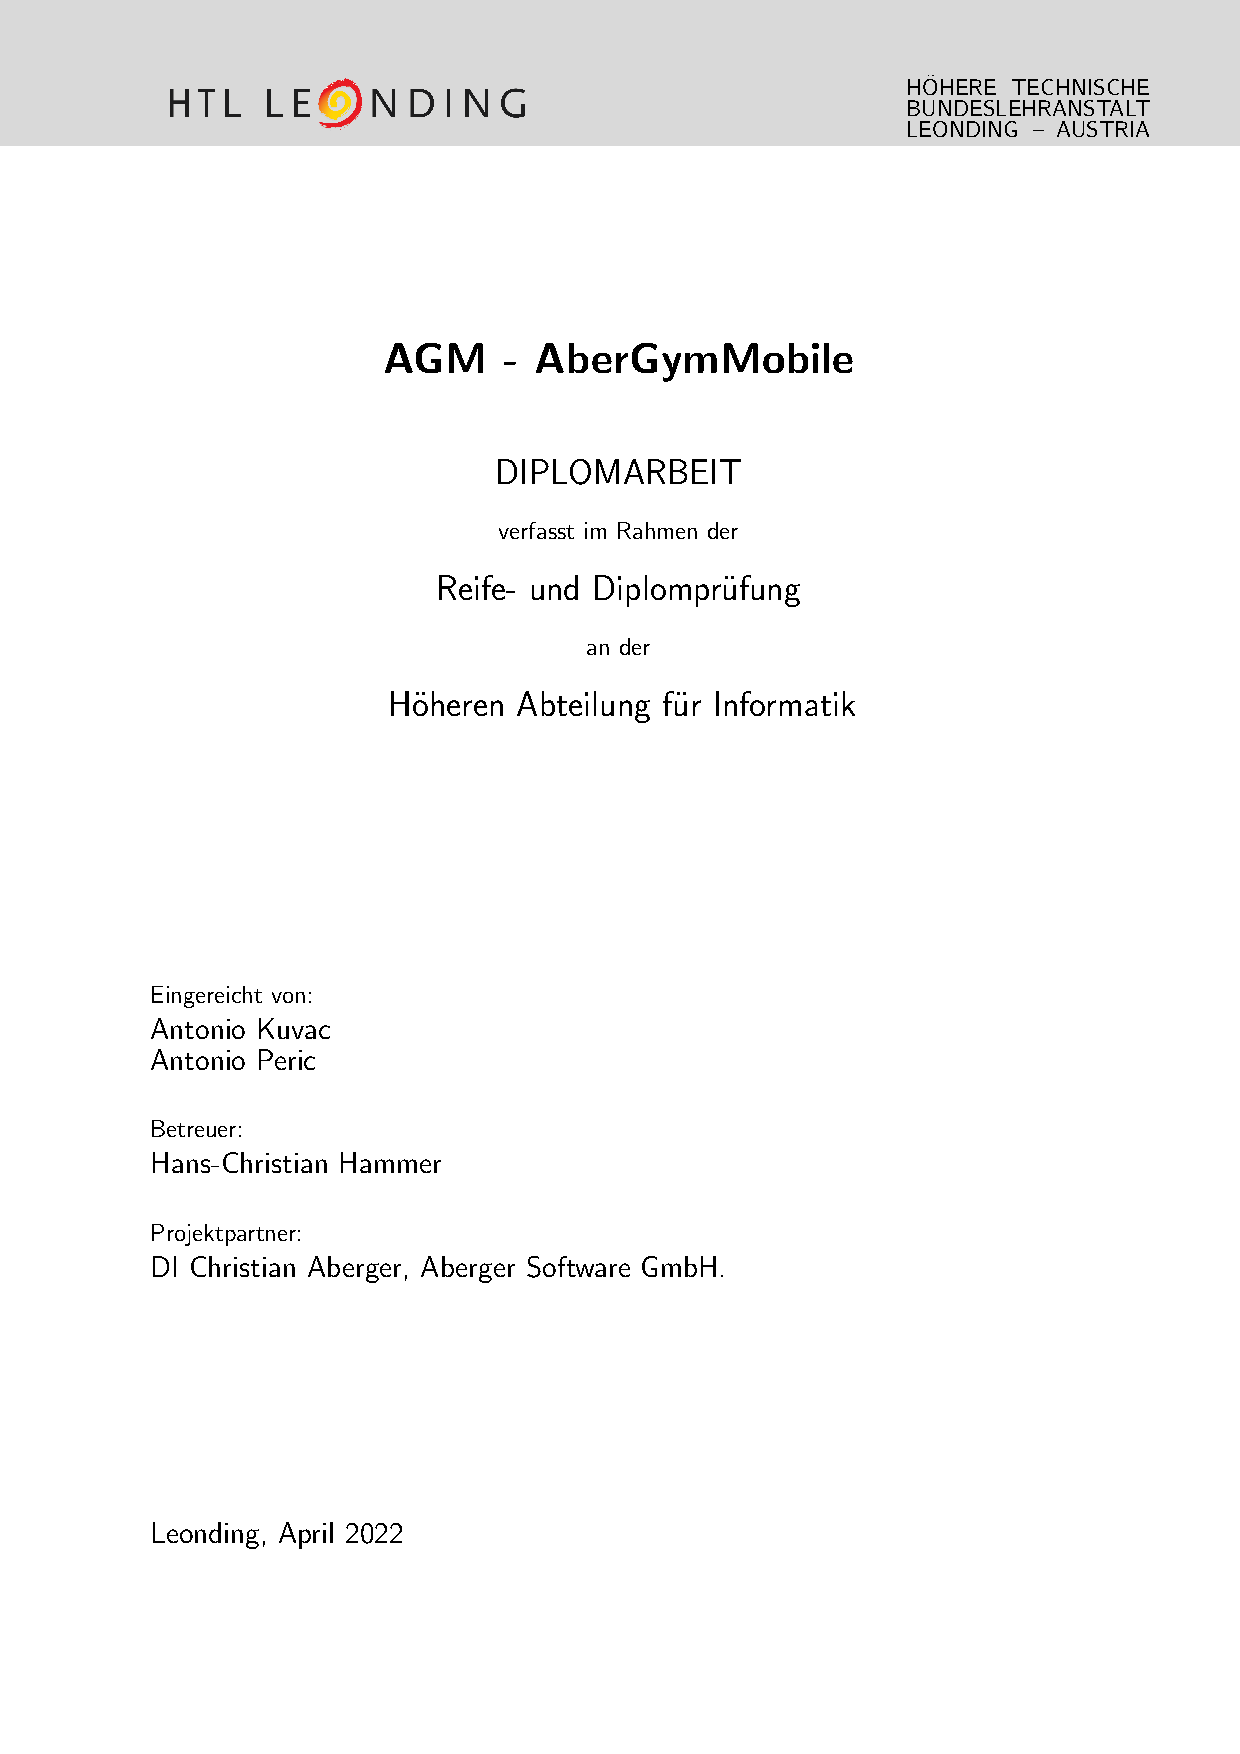
\includepdf{./titlepage/coversheet}
\pagenumbering{Roman}
\newpage
\thispagestyle{empty}
\vspace{3cm}
~ \\ \\
Ich erkläre an Eides statt, dass ich die vorliegende Diplomarbeit selbstständig und ohne fremde Hilfe verfasst, andere als die angegebenen Quellen und Hilfsmittel nicht benutzt bzw. die wörtlich oder sinngemäß entnommenen Stellen als solche kenntlich gemacht habe.

Die Arbeit wurde bisher in gleicher oder ähnlicher Weise keiner anderen Prüfungsbehörde vorgelegt und auch noch nicht veröffentlicht.

Die vorliegende Diplomarbeit ist mit dem elektronisch übermittelten Textdokument identisch.
\vspace{3cm}
% Hier kommt die Unterschrift drüber
\begin{tabbing}
Leonding, April 2022 \hspace{5cm} S. Schwammal \& S. Schwammal
\end{tabbing}
\vspace{10cm}
\newpage
\setcounter{page}{1}

\begin{spacing}{1}
    \chapter*{Abstract}
\end{spacing}
\begin{wrapfigure}{r}{0.3\textwidth}
    \begin{center}
      
\includegraphics[width=0.2\textwidth]{pics/question_mark.png}
    \end{center}
\end{wrapfigure}
Brief summary of our amazing work. In English.
This is the only time we have to include a picture within the text.
The picture should somehow represent your thesis.
This is untypical for scientific work but required by the powers that are.
\lipsum[6]
\newpage
\begin{spacing}{1}
    \chapter*{Zusammenfassung}
\end{spacing}
\begin{wrapfigure}{r}{0.3\textwidth}
    \begin{center}
      
\includegraphics[width=0.2\textwidth]{pics/question_mark.png}
    \end{center}
\end{wrapfigure}
Zusammenfassung unserer genialen Arbeit. Auf Deutsch.
Das ist das einzige Mal, dass eine Grafik in den Textfluss eingebunden wird.
Die gewählte Grafik soll irgendwie eure Arbeit repräsentieren.
Das ist ungewöhnlich für eine wissenschaftliche Arbeit aber eine Anforderung der Obrigkeit.
\emph{Bitte auf keinen Fall mit der Zusammenfassung verwechseln, die den Abschluss der Arbeit bildet!}
\lipsum[6]


\pagestyle{plain}

\renewcommand{\lstlistlistingname}{Quellcodeverzeichnis}

\tableofcontents
\newpage
\setcounter{RPages}{\value{page}}
\setcounter{page}{0}
\pagenumbering{arabic}
\pagestyle{scrheadings}

\begin{spacing}{1}
\chapter{Einleitung}\label{chapter:introduction}
\end{spacing}
\lipsum[2-3]

\begin{spacing}{1}
\chapter{Umfeldanalyse}
\end{spacing}
\lipsum[4] Citing \cite{InfH} properly.

Was ist eine \gls{guid}?
Eine \gls{guid} kollidiert nicht gerne.

Kabellose Technologien sind in abgelegenen Gebieten wichtig \cite{APCW2006}.


\begin{spacing}{1}
\chapter{Technologien}\label{chapter:tech}
\end{spacing}
\section{Flutter}
\setauthor{Antonio Peric}

Flutter ist ein Open-Source UI-Toolkit von Google zur Entwicklung von Anwendungen für mobile Geräte, Desktop-Computer und das Web. Es basiert auf der Programmiersprache Dart und verwendet eine Vielzahl von Widgets und Tools, um eine schnelle Entwicklung und hohe Qualität zu ermöglichen. Flutter ermöglicht es Entwicklern, attraktive und benutzerfreundliche Anwendungen zu erstellen, die auf verschiedenen Plattformen laufen können 
\cite{aws-flutter}.
\subsection{Entwicklungs-Ergonomie}

Flutter bietet eine sehr gute Entwicklungs-Ergonomie durch eine intuitive Benutzeroberfläche und eine umfassende Dokumentation. Die Widgets und Tools von Flutter sind gut strukturiert und können einfach angepasst werden. Darüber hinaus ermöglicht Flutter eine schnelle Erstellung von Prototypen und eine schnelle Iteration, was die Entwicklung von Anwendungen beschleunigt.

\subsection{Tiefgehende Codeanalyse}

Flutter bietet tiefgehende Codeanalysefunktionen, die Entwicklern helfen, Fehler schnell zu finden und zu beheben. Die Analysefunktionen umfassen eine statische Analyse, die Probleme wie Typfehler, fehlende Importe und andere Fehler aufdeckt, bevor die Anwendung ausgeführt wird. Flutter bietet auch eine dynamische Analyse, die Probleme während der Laufzeit aufdeckt.
\newpage

\subsection{Effiziente Navigation und Suche}

Flutter bietet eine effiziente Navigation und Suche, die es Entwicklern ermöglicht, schnell durch den Code zu navigieren und Probleme zu finden. Die IDEs, die Flutter unterstützen, wie beispielsweise IntelliJ IDEA, Visual Studio Code und Android Studio, bieten eine schnelle Navigation durch den Code sowie eine leistungsstarke Suche nach Dateien und Zeilen.

\subsection{Entwicklung: Ausführen, Testen, Debuggen}

Flutter ermöglicht Entwicklern eine effiziente Entwicklung, indem es ein integriertes Debugging- und Test-Framework bietet. Entwickler können ihre Anwendungen in Echtzeit testen und debuggen, ohne die Anwendung manuell neu starten zu müssen. Das Testen von Anwendungen ist ebenfalls einfach und kann durch den Einsatz von Frameworks wie Flutter Test und Mockito unterstützt werden.

\subsection{Funktionen}

Flutter bietet zahlreiche Funktionen und Tools, um Entwicklern bei der Entwicklung von Anwendungen zu helfen. Hier sind einige der wichtigsten Funktionen:

\begin{itemize}
\item Widgets: Flutter bietet eine große Auswahl an vorgefertigten Widgets, die Entwickler verwenden können, um benutzerdefinierte Benutzeroberflächen zu erstellen.
\item Hot Reload: Mit Hot Reload können Entwickler Änderungen an der Anwendung vornehmen und diese Änderungen sofort überprüfen, ohne die Anwendung neu starten zu müssen.
\item State Management: Flutter bietet eine Vielzahl von State-Management-Lösungen, einschließlich Provider und Redux, die es Entwicklern ermöglichen, den Zustand ihrer Anwendung effizient zu verwalten.
\item Plattformunabhängigkeit: Flutter ist plattformunabhängig und ermöglicht es Entwicklern, eine Anwendung zu erstellen, die auf verschiedenen Plattformen ausgeführt werden kann, einschließlich Android, iOS, Web und Desktop.
\newpage
\item Performance: Flutter ist schnell und leistungsfähig und bietet eine schnelle Animation und flüssige Benutzeroberflächen, ohne Einbußen bei der Performance. Durch die Verwendung von Skia, einer 2D-Grafik-Engine, können Entwickler hochwertige Animationen und visuell ansprechende Benutzeroberflächen erstellen, die auf verschiedenen Geräten einheitlich und flüssig funktionieren.
\end{itemize}

\subsection{Vorteile}
Flutter bietet mehrere Vorteile:

\begin{compactitem}
    \item \textbf{Plattformübergreifende Entwicklung}: Mit Flutter können Entwickler plattformübergreifende Anwendungen erstellen, die auf verschiedenen Betriebssystemen wie iOS, 
    Android, Web und Desktop laufen. Dies reduziert die Entwicklungskosten und spart Zeit und Ressourcen.
    \item \textbf{Schnelle Entwicklung}: Flutter bietet die Funktion "Hot Reload", die es Entwickler*innen ermöglicht, Änderungen in Echtzeit zu sehen, 
    ohne die Anwendung neu starten zu müssen. Dadurch wird die Entwicklung von Flutter-Anwendungen schneller und effizienter.
    \item \textbf{Reaktionsfähigkeit}: Flutter-Anwendungen sind schnell und reaktionsfähig, da sie auf der leistungsstarken Grafik-Engine Skia basieren. 
    Dies ermöglicht es Entwickler*innen, reibungslose Benutzererfahrungen mit flüssigen Animationen und Grafiken zu schaffen.
    \item \textbf{Einfache UI-Erstellung}: Mit der eigenen Widget-Bibliothek von Flutter können Entwickler*innen schnell und einfach ansprechende Benutzeroberflächen erstellen. 
    Die Bibliothek enthält viele vorgefertigte Widgets, die einfach angepasst werden können.
    \item \textbf{Native Performance}: Flutter-Anwendungen werden in nativem Code ausgeführt, was zu einer höheren Leistung und Geschwindigkeit führt als bei Hybrid- oder webbasierten Anwendungen.
\end{compactitem}

\newpage
\section{Dart als Programmiersprache}
Dart ist eine objektorientierte Programmiersprache, die von Google entwickelt wurde und erstmals im Jahr 2011 vorgestellt wurde. Im Vergleich zu anderen Sprachen wie Java, Python und C++ ist Dart eine vergleichsweise neue Programmiersprache. Sie wurde entwickelt, um die Herausforderungen bei der Entwicklung von Webanwendungen zu bewältigen und ist auch für die Entwicklung von plattformübergreifenden mobilen Anwendungen geeignet \cite{aws-flutter}.

\subsection{Statische Typisierung}
Eine der wichtigsten Eigenschaften von Dart ist die statische Typisierung. Statische Typisierung bedeutet, dass Variablen und Funktionen vor der Laufzeit überprüft werden. Dadurch können Entwickler*innen Fehler frühzeitig erkennen und vermeiden. Statische Typisierung verbessert auch die Lesbarkeit und Wartbarkeit des Codes.

\subsection{Dynamische Typisierung}
Dart unterstützt auch dynamische Typisierung. Diese Funktion erleichtert die Entwicklung von Anwendungen, die auf sich ändernden Datenstrukturen basieren. Mit der dynamischen Typisierung kann der Code flexibler gestaltet werden und Entwickler*innen können schneller auf Änderungen reagieren.

\subsection{Funktionale Programmierung}
Dart unterstützt auch funktionale Programmierung, die eine saubere und lesbare Codebasis fördert. Die Verwendung von Funktionen als Parameter erhöht die Flexibilität und Wiederverwendbarkeit von Code.

\subsection{Asynchrone Programmierung}
Dart unterstützt asynchrone Programmierung, um die Leistung bei der Verarbeitung von Netzwerk- und E/A-Operationen zu verbessern. Mit der asynchronen Programmierung können Entwickler*innen Anwendungen entwickeln, die schnell und effizient arbeiten und auf die Bedürfnisse der*die Benutzer*innen reagieren.

\subsection{Widgets}

Ein zentraler Bestandteil von Flutter sind Widgets. Widgets sind die Bausteine für die Erstellung von Benutzeroberflächen in Flutter. Sie sind leichtgewichtig und anpassbar und ermöglichen es Entwicklern, komplexe Benutzeroberflächen mit wenig Code zu erstellen. Es gibt eine große Auswahl an vorgefertigten Widgets in Flutter, die Entwickler verwenden können, um schnell und einfach eine benutzerdefinierte Benutzeroberfläche zu erstellen.

Flutter bietet auch die Möglichkeit, eigene Widgets zu erstellen. Dies gibt Entwicklern mehr Flexibilität und Kontrolle über die Benutzeroberfläche ihrer Anwendung. Darüber hinaus können Widgets in Flutter einfach angepasst werden, um sie an die Anforderungen der Anwendung anzupassen.

\subsection{State Management}

Die Verwaltung des Zustands ist ein wichtiger Aspekt bei der Entwicklung von Anwendungen. In Flutter gibt es verschiedene Möglichkeiten, den Zustand einer Anwendung effizient zu verwalten. Die am häufigsten verwendeten Lösungen für das State Management in Flutter sind Provider und Redux.

Provider ist eine einfachere Lösung für das State Management, die es Entwicklern ermöglicht, den Zustand ihrer Anwendung zu verwalten, ohne zusätzliche Bibliotheken hinzufügen zu müssen. Es ist eine leichtgewichtige Lösung, die die Verwaltung des Zustands vereinfacht und die Leistung der Anwendung verbessert.

Redux ist eine robuste Lösung für das State Management in Flutter, die Entwicklern eine hohe Kontrolle über den Zustand ihrer Anwendung bietet. Redux ist eine Bibliothek, die es Entwicklern ermöglicht, den Zustand ihrer Anwendung zentralisiert zu verwalten. Es bietet auch eine Vielzahl von Werkzeugen und Funktionen, um die Verwaltung des Zustands zu erleichtern.
\newpage
\subsection{Vorteile von Dart}

Dart bietet eine Reihe von Vorteilen für Entwickler, darunter:

\begin{itemize}
\item \textbf{Effiziente Ausführung}: Dart ist eine schnelle und leistungsfähige Sprache, die eine effiziente Ausführung von Anwendungen ermöglicht.
\item \textbf{Statische Typisierung}: Dart ist eine statisch typisierte Sprache, die Entwicklern hilft, Fehler frühzeitig zu erkennen und zu beheben.
\item \textbf{Flexibilität}: Dart unterstützt dynamische Typisierung, was Entwicklern Flexibilität bei der Entwicklung von Anwendungen bietet, die auf sich ändernden Datenstrukturen basieren.
\item \textbf{Asynchrone Programmierung}: Dart unterstützt asynchrone Programmierung, um die Leistung bei der Verarbeitung von Netzwerk- und E/A-Operationen zu verbessern.
\item \textbf{Wiederverwendbarkeit von Code}: Dart bietet die Möglichkeit, Funktionen als Parameter zu übergeben, um die Wiederverwendbarkeit von Code zu erhöhen.
\item \textbf{Einfach zu erlernen}: Dart ist eine relativ einfache Sprache, die schnell erlernt werden kann.
\item \textbf{Integration mit Flutter}: Dart wird von Flutter unterstützt und bietet Entwicklern eine leistungsstarke und effiziente Möglichkeit, plattformübergreifende Anwendungen zu entwickeln.
\end{itemize}

\pagebreak
\section{Visual Studio Code}
\setauthor{Antonio Kuvac}
Visual Studio Code ist ein kostenloses, plattformübergreifendes Code-Editor-Tool von Microsoft. Es ist ein beliebtes Tool für Entwickler*innen, 
da es eine Vielzahl von Funktionen und Erweiterungen bietet, um die Produktivität und Effizienz zu verbessern.

Visual Studio Code bietet eine intuitive Benutzeroberfläche, die es Entwickler*innen erleichtert, schnell und einfach zu navigieren und Code zu schreiben. 
Es bietet auch integrierte Debugging-Tools, die Entwickler*innen helfen, Fehler zu finden und zu beheben, sowie integrierte Versionskontrolltools für Git, 
um Änderungen am Code effektiv zu verwalten.

\subsection{Extensions}
Eine der wesentlichsten Funktionen in VS Code sind Extensions (Erweiterungen). VS Code-Extensions können verschiedene Funktionen bieten, 
wie z.B. Syntax-Hervorhebung, Autovervollständigung, Debugging-Tools, Git-Integration und vieles mehr. 
Es gibt eine breite Palette von Erweiterungen, die für verschiedene Programmiersprachen und Frameworks verfügbar sind, 
um die Entwicklungserfahrung zu verbessern und die Produktivität zu steigern.

Die Installation von VS Code-Extensions ist einfach und unkompliziert. Sie können über den Visual Studio Code-Marktplatz oder direkt aus der Editor-Benutzeroberfläche installiert werden.
Nach der Installation stehen die neuen Funktionen und Tools sofort zur Verfügung.
\pagebreak
\section{Docker}
\setauthor{Antonio Kuvac}
Docker ist eine Open-Source-Plattform, die es Entwicklern ermöglicht, Anwendungen in isolierten Containern zu erstellen, bereitzustellen und auszuführen. 
Docker-Container sind leichtgewichtig und portabel und bieten eine effektive Möglichkeit, Anwendungen in verschiedenen Umgebungen und Infrastrukturen auszuführen.

\subsection{Funktionsweise}
Docker verwendet Container, um Anwendungen zu isolieren und eine konsistente Umgebung für ihre Ausführung zu schaffen. Container sind ähnlich wie virtuelle Maschinen, 
jedoch leichter und schneller zu erstellen, da sie den Kernel des Host-Betriebssystems nutzen. Jeder Container enthält alles, was eine Anwendung zum Ausführen benötigt, 
einschließlich des Codes, der Abhängigkeiten und der Konfiguration.

Die Funktionsweise von Docker basiert auf einem Schichtmodell, das aus drei Komponenten besteht:

\begin{enumerate}
    \item \textbf{Docker Engine}: Dies ist das Kernstück von Docker und besteht aus dem Docker-Daemon und der Docker-CLI (Command Line Interface). Der Docker-Daemon ist ein Hintergrundprozess, 
    der die Verwaltung und Ausführung von Containern übernimmt, während die Docker-CLI als Schnittstelle für den Benutzer dient, um mit dem Docker-Daemon zu interagieren.
    \item \textbf{Images}: Ein Docker-Image ist eine Vorlage oder Blaupause für die Erstellung von Containern. 
    Es enthält den Code, die Abhängigkeiten und Konfigurationen einer Anwendung sowie alle anderen erforderlichen Komponenten, die zur Ausführung der Anwendung benötigt werden. 
    Docker-Images werden über Docker Files erstellt, die eine Liste von Anweisungen enthalten, um das Image zu konfigurieren und zu erstellen.
    \item \textbf{Container}: Ein Docker-Container ist eine Instanz eines Docker-Images, die ausgeführt wird. Ein Container kann gestartet, gestoppt und gelöscht werden. 
    Jeder Container ist isoliert und hat seine eigene Dateisystemumgebung, Netzwerkschnittstellen und Ressourcenlimits.
    \end{enumerate}

    \begin{figure}[H]
        \centering
        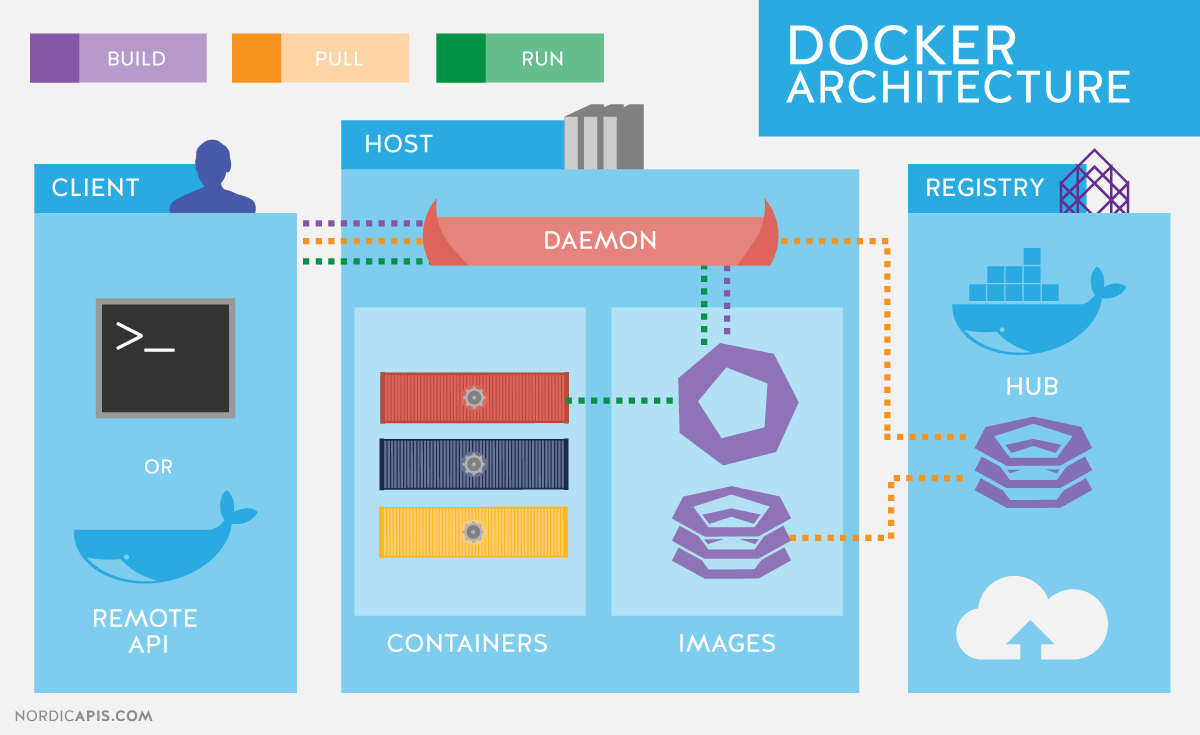
\includegraphics[scale=0.3]{pics/Docker_Architecture.png}
        \caption{Docker Architektur}
    \end{figure}

\subsection{Vorteile}
\begin{itemize}
    \item \textbf{Portabilität}: Docker-Container sind plattformunabhängig und können auf verschiedenen Betriebssystemen und Infrastrukturen ausgeführt werden.
    
    \item \textbf{Flexibilität}: Mit Docker können Anwendungen schnell erstellt, abgeändert und bereitgestellt werden, ohne die zugrunde liegende Infrastruktur ändern zu müssen.
    
    \item \textbf{Skalierbarkeit}: Docker ermöglicht eine einfache horizontale Skalierung von Anwendungen, indem es das Erstellen und Bereitstellen von Containern automatisiert.
    
    \item \textbf{Sicherheit}: Docker bietet Sicherheitsfunktionen wie Isolation und eingeschränkte Ressourcenkontrolle, um eine sicherere Ausführung von Anwendungen zu gewährleisten.
    
    \item \textbf{Effizienz}: Docker-Container sind leicht und benötigen weniger Ressourcen als virtuelle Maschinen, was zu einer höheren Effizienz und Leistung führt.
    \end{itemize}

    \section{Android Studio}
    \setauthor{Antonio Kuvac}
    Android Studio ist eine integrierte Entwicklungsumgebung (IDE), die speziell für die Entwicklung von Android-Apps entwickelt wurde. 
    Es wurde von Google entwickelt und ist kostenlos für Entwickler verfügbar, um Android-Apps zu erstellen und zu bearbeiten.

    \subsection{Funktionen}
    Android Studio verfügt über eine Vielzahl von Funktionen, die dabei helfen, schneller und effizienter Android-Apps zu entwickeln. Zu den wichtigsten Funktionen gehören:

    \begin{itemize}
        \item \textbf{Intelligentes Code-Editing:} Android Studio bietet intelligentes Code-Editing mit automatischen Vorschlägen, Fehlererkennung und Refactoring-Funktionen.
        \item \textbf{Emulator:} Entwickler können den Android-Emulator nutzen, um ihre Apps auf verschiedenen Android-Geräten zu testen, ohne physische Geräte besitzen zu müssen.
        \item \textbf{Layout-Editor:} Android Studio verfügt über einen Layout-Editor, mit dem Entwickler die Benutzeroberfläche ihrer Apps visuell gestalten können.
        \item \textbf{Gradle Build-System:} Android Studio verwendet das Gradle Build-System, das Entwicklern ermöglicht, komplexe Abhängigkeiten und Builds zu verwalten.
        \item \textbf{Integration mit anderen Tools:} Android Studio ist nahtlos in andere Google-Tools wie Firebase und Google Cloud Platform integriert.
        \end{itemize}

    \subsection{Emulator}
    Der Android Studio Emulator ist ein wichtiges Tool für Android-Entwickler, das es ihnen ermöglicht, ihre Apps auf verschiedenen Android-Geräten zu testen, ohne physische Geräte besitzen zu müssen. Der Emulator wird mit Android Studio mitgeliefert und kann einfach über die IDE gestartet werden.

Einer der größten Vorteile des Emulators ist, dass Entwickler ihre Apps auf verschiedenen Android-Versionen und Gerätekonfigurationen testen können, um sicherzustellen, 
dass ihre Apps auf allen unterstützten Geräten reibungslos funktionieren. 
Der Emulator kann eine Vielzahl von Android-Versionen und -Gerätekonfigurationen emulieren, einschließlich verschiedener Bildschirmauflösungen und -größen, 
Prozessortypen und Speicherkapazitäten.

Ein weiterer Vorteil des Emulators ist, dass er den Entwicklungsprozess beschleunigen kann, indem er den Build- und Bereitstellungsprozess verkürzt. 
Anstatt jedes Mal eine neue Version der App auf einem physischen Gerät zu testen, können Entwickler die App einfach im Emulator starten und testen, 
was Zeit spart und die Entwicklungszeit verkürzt.

Die Einrichtung des Emulators in Android Studio ist einfach und erfordert nur wenige Schritte. Entwickler müssen zunächst sicherstellen, 
dass sie die neueste Version von Android Studio heruntergeladen und installiert haben. Sobald sie Android Studio geöffnet haben, können sie den Emulator über das AVD Manager-Tool starten, 
das im Menü "Werkzeuge" zu finden ist.

Es gibt jedoch auch einige Nachteile beim Verwenden des Emulators. Einer der größten Nachteile ist die Geschwindigkeit. Da der Emulator ein virtuelles Gerät ist, 
kann er langsamer sein als ein physisches Gerät. Dies kann dazu führen, dass Entwickler länger warten müssen, um ihre Apps im Emulator zu testen.

Ein weiterer Nachteil ist, dass der Emulator nicht alle Funktionen eines physischen Geräts emulieren kann. Beispielsweise kann der Emulator keine Anrufe oder Textnachrichten empfangen und senden, 
da er kein physisches Mobilfunkmodem hat. Dies bedeutet, dass Entwickler nicht alle Aspekte ihrer App im Emulator testen können und gegebenenfalls auf physische Geräte zurückgreifen müssen.

Zusammenfassend lässt sich sagen, dass der Android Studio Emulator ein wertvolles Tool für Android-Entwickler ist, um ihre Apps auf verschiedenen Geräten und Android-Versionen zu testen. 
Obwohl der Emulator einige Nachteile hat, überwiegen die Vorteile in den meisten Fällen und er ist ein unverzichtbares Werkzeug für die App-Entwicklung.

\begin{figure}[H]
    \centering
    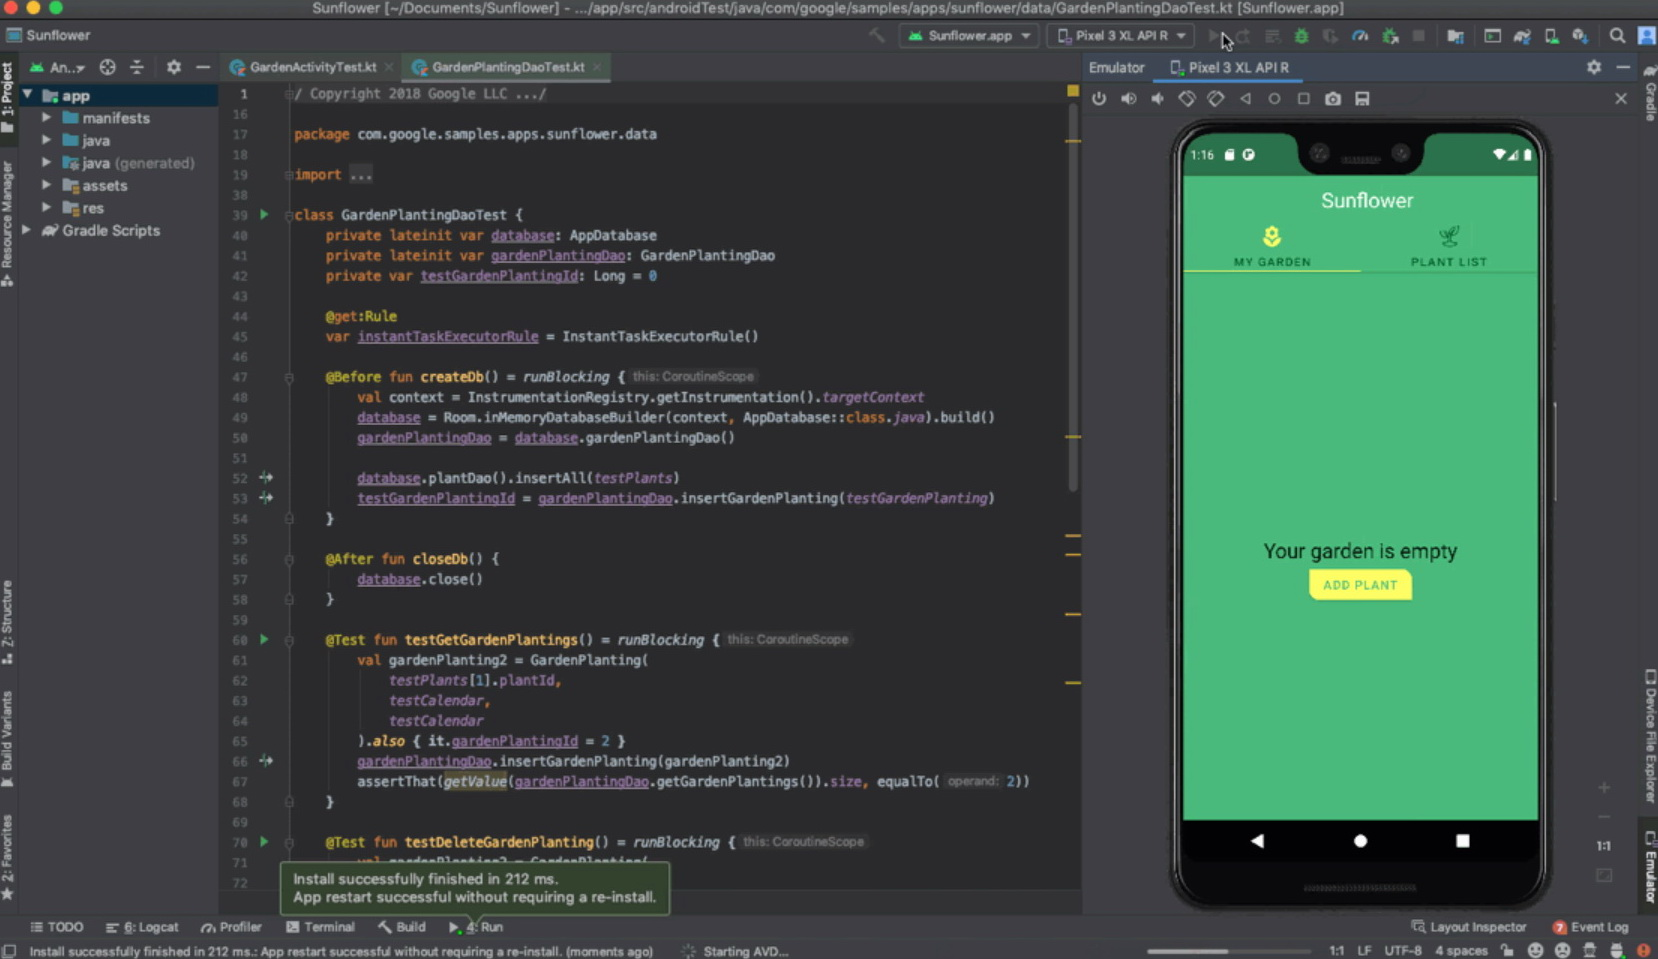
\includegraphics[scale=0.2]{pics/android-studio-emulator.jpg}
    \caption{Android Studio Emulator}
\end{figure}

\section{AdobeXD}
    \setauthor{Antonio Kuvac}

    AdobeXD ist eine Design-Software, die speziell für die Erstellung von Benutzeroberflächen und Interaktionen für Mobile Apps, Webseiten und andere digitale Plattformen entwickelt wurde.

\subsection*{Funktionen}
Die wichtigsten Funktionen sind intuitive Layout-Tools, um Entwürfe schnell zu erstellen und zu bearbeiten, Vektor-Tools, um hochwertige Grafiken zu erstellen, Prototyping-Funktionen, um interaktive Prototypen zu erstellen und zu testen und die Möglichkeit, Designs in Echtzeit zu teilen und Feedback von Stakeholdern zu erhalten.

\subsection*{Plattformübergreifendes Design} 
AdobeXD unterstützt plattformübergreifendes Design, was bedeutet, dass man nur eine einzige Design-Datei erstellen muss, um diese dann auf AdobeXD auf verschiedenen Geräten und Plattformen verwenden zu können. 
Das ermöglicht, schnell und effizient Designs für verschiedene Geräte und Plattformen zu erstellen.

\subsection*{Integration mit anderen Tools} 
AdobeXD ist nahtlos in andere Adobe-Tools wie Photoshop und Illustrator integriert. Das ermöglicht, Designs nahtlos zwischen verschiedenen Adobe-Tools zu übertragen. 
Es ist auch in andere Tools wie Slack und Microsoft Teams integriert, um die Zusammenarbeit zu erleichtern.

\subsection*{Cloud-basierte Zusammenarbeit} 
AdobeXD bietet eine Cloud-basierte Zusammenarbeit an, mit der es möglich ist, Designs in Echtzeit zu teilen und Feedback von Stakeholdern zu erhalten. 
Designer*innen können Links zu ihren Designs freigeben und Stakeholder können Kommentare und Feedback direkt in die Designs geben.

\section{IntelliJ IDEA}
\setauthor{Antonio Peric}

\textbf{IntelliJ IDEA} ist eine leistungsstarke und vielseitige Entwicklungsumgebung, die von Entwicklern auf der ganzen Welt genutzt wird. Mit der Fähigkeit, eine Vielzahl von Programmiersprachen zu unterstützen, hat es sich zu einem wichtigen Werkzeug für die Softwareentwicklung entwickelt.

Die Free-Version von IntelliJ IDEA bietet Unterstützung für Programmiersprachen wie Java, Groovy, Kotlin und Scala sowie Standardsyntaxsprachen wie XML. Mit dieser Version können Entwickler grundlegende Projekte erstellen und debuggen. Die Ultimate-Version von IntelliJ IDEA bietet jedoch erweiterte Funktionen, wie beispielsweise die Integration mit Frameworks, eine größere Auswahl an Plugins, Code-Refactoring-Tools und viele weitere Funktionen, die die Produktivität von Entwicklern erhöhen.

Für Schüler*innen und Studenten*innen steht die Ultimate-Version von IntelliJ IDEA zu einem reduzierten Preis zur Verfügung, was ihnen den Zugang zu leistungsstarken Werkzeugen zur Entwicklung von Anwendungen ermöglicht. Zudem ist es möglich, durch kostenlose Community- oder offizielle Jetbrains-Plugins, weitere Programmiersprachen in IntelliJ IDEA zu integrieren, wie Go, Python, SQL, Ruby und PHP \cite{IntelliJ}.

\subsection{Entwicklungs-Ergonomie}
Die IntelliJ IDEA Ultimate bietet zahlreiche Optionen zur Erstellung neuer Projekte und ermöglicht so einen einfachen Einstieg in die Entwicklung. Individuelle Anpassungen wie das Ändern des Designs oder der Tastenkürzel sind möglich, um die IDE an die Bedürfnisse des Entwicklers anzupassen. Zusätzliche Funktionalitäten können durch Plugins hinzugefügt werden, um spezifische Anforderungen zu erfüllen.
\newpage

\subsection{Tiefgehende Codeanalyse}
Obwohl die IntelliJ Ultimate IDE hauptsächlich für die Java-Entwicklung entwickelt wurde, unterstützt sie auch eine Vielzahl anderer Programmiersprachen wie Groovy, Kotlin, Scala, JavaScript, TypeScript und SQL. Für jede dieser Sprachen bietet die IntelliJ IDEA eine spezielle intelligente Programmierhilfe. Durch die Indexierung des Projektcodes beim Start der IDE können Fehler während der Entwicklung in Echtzeit erkannt und Code-Vervollständigungsvorschläge angezeigt werden. Zusätzlich bietet die IDE Funktionen zur Durchführung von Refactorings, wie zum Beispiel Umbenennung von Dateinamen.

\subsection{Effiziente Navigation und Suche}
Die IntelliJ IDEA ermöglicht es dem Benutzer, schnell und einfach nach bestimmten Wörtern im gesamten Projekt zu suchen, indem eine Globale Suche verwendet wird. Alternativ kann auch eine Lokale Suche in der aktuellen Datei durchgeführt werden. Wenn ein Wort in einer Datei ausgewählt wird, werden alle anderen Vorkommen dieses Wortes in der Datei hervorgehoben. Zusätzlich können Funktionen und Klassen in ihrem Kontext betrachtet werden, indem jede Verwendung dieser Elemente dargestellt wird. Dies erleichtert die Navigation und Verwaltung von Code in großen Projekten.

\subsection{Entwicklung: Ausführen, Testen, Debuggen}
Für das Ausführen von Projekten kann in IntelliJ IDEA das integrierte Terminal genutzt werden. Alternativ dazu bietet die IDE auch die Möglichkeit, Projekte direkt innerhalb der Entwicklungsumgebung auszuführen. Hierfür können verschiedene Zielplattformen definiert werden, auf denen das Projekt laufen soll. Des Weiteren bietet die IDE eine umfangreiche Unterstützung für Code-Tests und Debugging-Funktionen an.
\newpage

\subsection{Effektive Zusammenarbeit im Team}
Durch Code With Me von Jetbrains können mehrere Personen in Echtzeit an einer gemeinsamen Datei arbeiten. Zusätzlich können Video- und Sprachanrufe über die Plattform getätigt werden, um sich mit anderen Teammitgliedern zu besprechen. Des Weiteren hat Jetbrains kürzlich ein Remote-Development-System eingeführt, welches es ermöglicht, die IntelliJ Ultimate IDEA auf einem leistungsstarken Host-System zu betreiben. Über dieses neue Tool können Nutzer von überall auf der Welt auf ihre Projekte zugreifen und von verschiedenen Orten aus gemeinsam arbeiten.

\subsection{Funktionen}

Die Entwicklungsumgebung IntelliJ bietet zahlreiche Funktionen und Tools, um Entwickler*innen bei der Entwicklung von Softwareprojekten zu unterstützen. Nachfolgend sind einige der wichtigsten Funktionen aufgeführt:

\begin{itemize}
\item Code-Editing: IntelliJ bietet intelligentes Code-Editing mit Code-Vervollständigung, Syntax-Hervorhebung, Refactoring und Code-Analyse-Funktionen.
\item Debugger: Der integrierte Debugger ermöglicht es Entwicklerinnen, Code zu debuggen und Fehler schnell zu finden.
\item Build-Tools: IntelliJ unterstützt eine Vielzahl von Build-Tools wie Gradle, Maven und Ant.
\item Integration mit anderen Tools: IntelliJ ist nahtlos in andere Tools und Frameworks wie Git, JUnit und Spring integriert.
\item Version-Control-System: IntelliJ unterstützt verschiedene Version-Control-Systeme wie Git, Subversion und Mercurial.
\item Code-Qualität: IntelliJ bietet Code-Qualität-Tools, um Entwicklerinnen dabei zu helfen, fehlerfreien Code zu schreiben und Code-Qualitätsstandards einzuhalten.
\item Frameworks: IntelliJ unterstützt eine Vielzahl von Frameworks wie Spring, Hibernate, Struts und mehr.
\end{itemize}
\newpage

\subsection{Vorteile}

IntelliJ bietet eine Vielzahl von Vorteilen für Entwickler, darunter:

\begin{itemize}
    \item Code-Refactoring: IntelliJ bietet eine Vielzahl von Code-Refactoring-Tools, mit denen Entwickler Code effizienter und strukturierter gestalten können.
    \item Automatisierte Tests: IntelliJ unterstützt automatisierte Tests, die Entwicklern helfen, Fehler frühzeitig zu erkennen und zu beheben.
    \item Plugins: IntelliJ hat eine große Auswahl an Plugins, die Entwickler verwenden können, um ihre Arbeitsumgebung zu erweitern und ihre Produktivität zu steigern.
    \item Gute Performance: IntelliJ ist bekannt für seine gute Performance und Stabilität, was Entwicklern ermöglicht, effizienter zu arbeiten.
    \item Unterstützung für Cloud-Computing: IntelliJ ist auch in der Lage, mit Cloud-Computing-Plattformen wie Amazon Web Services, Google Cloud Platform und Microsoft Azure zu arbeiten.
    \item Mobile App-Entwicklung: IntelliJ bietet Unterstützung für die Entwicklung von mobilen Apps für Android und iOS, einschließlich Integrationen mit Android Studio und Xcode.
\end{itemize}

\begin{spacing}{1}
\chapter{Umsetzung}\label{chapter:implementation}
\end{spacing}
Siehe tolle Daten in Tab. \ref{tab:impl:data}.

\begin{table}
    \centering
    \begin{tabular}{|lcc|}
    \hline
              & \textbf{Regular Customers} & \textbf{Random Customers} \\ \hline
    Age       & 20-40                      & \textgreater{}60          \\ \hline
    Education & university                 & high school               \\ \hline
    \end{tabular}
    \caption{Ein paar tabellarische Daten}
    \label{tab:impl:data}
\end{table}

\begin{figure}
    \centering
    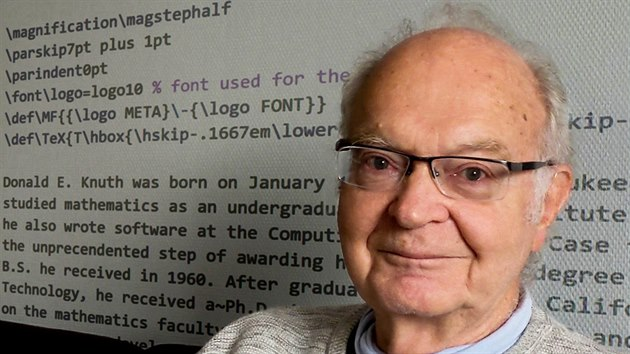
\includegraphics[scale=0.5]{pics/knuthi.jpg}
    \caption{Don Knuth -- CS Allfather}
    \label{fig:impl:knuth}
\end{figure}

Siehe und staune in Abb. \ref{fig:impl:knuth}.
\lipsum[6-9]
Dann betrachte den Code in Listing \ref{lst:impl:foo}.

\begin{lstlisting}[language=Python,caption=Some code,label=lst:impl:foo]
# Program to find the sum of all numbers stored in a list (the not-Pythonic-way)

# List of numbers
numbers = [6, 5, 3, 8, 4, 2, 5, 4, 11]

# variable to store the sum
sum = 0

# iterate over the list
for val in numbers:
    sum = sum+val

print("The sum is", sum)
\end{lstlisting}

\begin{spacing}{1}
\chapter{Zusammenfassung}
\end{spacing}
Aufzählungen:

\begin{compactitem}
    \item Itemize Level 1
    \begin{compactitem}
        \item Itemize Level 2
        \begin{compactitem}
            \item Itemize Level 3 (vermeiden)
        \end{compactitem}
    \end{compactitem}
\end{compactitem}

\begin{compactenum}
    \item Enumerate Level 1
    \begin{compactenum}
        \item Enumerate Level 2
        \begin{compactenum}
            \item Enumerate Level 3 (vermeiden)
        \end{compactenum}
    \end{compactenum}
\end{compactenum}

\begin{compactdesc}
    \item[Desc] Level 1
    \begin{compactdesc}
        \item[Desc] Level 2 (vermeiden)
        \begin{compactdesc}
            \item[Desc] Level 3 (vermeiden)
        \end{compactdesc}
    \end{compactdesc}
\end{compactdesc}

\newpage
\pagenumbering{Roman}
\setcounter{page}{\value{RPages}}
\newacronym{guid}{GUID}{Globally Unique Identifier}
\newacronym{jit}{JIT}{Just In Time Compiler}
\newacronym{nfc}{NFC}{Near Field Communication}
\newacronym{rfid}{RFID}{Radio Frequency Identification}

% Usage:
% \gls{label} lowercase in text
% \Gls{label} Uppercase in text
% \newacronym{label}{abbrev}{full}
% \newglossaryentry{label}{settings}



%\setlength{\glsdescwidth}{0.8\linewidth}
\glsnogroupskiptrue
\printglossary[title=Glossar,toctitle=Glossar] %,style=long]
\spacing{1}{
%\bibliographystyle{IEEEtran}
\bibliographystyle{ieeetrande}
\bibliography{bib}
}
\listoffigures
\listoftables
\lstlistoflistings
\appendix
\addchap{Anhang}
\input{./sections/appendix}
\end{document}

